\whiteBGstarBegin
\setcounter{section}{0}
\section{Trắc nghiệm}
\begin{enumerate}[label=\bfseries Câu \arabic*:]
	
	
	\item \mkstar{1}
	
	\cauhoi
	{Chọn câu đúng.
		\begin{mcq}
			\item Cường độ dòng điện trong mạch kín tỉ lệ nghịch với điện trở ngoài của nguồn.
			\item Cường độ dòng điện trong mạch kín tỉ lệ nghịch với suất điện động của nguồn.
			\item Cường độ dòng điện trong mạch kín tỉ lệ nghịch với điện trở trong của nguồn.
			\item Cường độ dòng điện trong mạch kín tỉ lệ nghịch với tổng điện trở toàn mạch.
		\end{mcq}
		
	}
	\loigiai
	{	\textbf{Đáp án: D.}
		
		Cường độ dòng điện trong mạch kín tỉ lệ nghịch với tổng điện trở toàn mạch:
		$$I=\dfrac{\calE}{R+r}.$$
	}
	\item \mkstar{1}
	
	\cauhoi
	{Công thức nào dưới đây là định luật Ôm toàn mạch?
		\begin{mcq}(2)
			\item $I=\dfrac{\calE}{R+r}$.
			\item $U_\text{AB} = \calE - Ir$.
			\item $U_\text{AB} = \calE + Ir$.
			\item $U_\text{AB} = I_\text{AB} (R+r) - \calE$.
		\end{mcq}
		
	}
	\loigiai
	{	\textbf{Đáp án: A.}
		
		Cường độ dòng điện trong mạch kín tỉ lệ nghịch với tổng điện trở toàn mạch:
		$$I=\dfrac{\calE}{R+r}.$$
	}
	\item \mkstar{2}
	
	\cauhoi
	{Một nguồn điện có suất điện động 10 V và điện trở trong $\SI{1}{\Omega}$. Mắc nguồn điện với điện trở ngoài $\SI{4}{\Omega}$. Cường độ dòng điện trong mạch có độ lớn bằng
		\begin{mcq}(4)
			\item 10 A.
			\item $\SI{2.5}{A}$.
			\item 2 A.
			\item 4 A.
		\end{mcq}
		
	}
	\loigiai
	{	\textbf{Đáp án: C.}
		
		Áp dụng công thức:
		$$I=\dfrac{\calE}{R+r} = \SI{2}{A}.$$
	}
	\item \mkstar{2}
	
	\cauhoi
	{Theo định luật Ôm toàn mạch, khi thay đổi điện trở ngoài $R$ thì đồ thị biểu diễn sự phụ thuộc của hiệu điện thế giữa hai cực của nguồn vào cường độ dòng điện trong mạch có dạng
		\begin{mcq}
			\item một đoạn thẳng đi qua gốc tọa độ.
			\item một phần của đường parabol.
			\item một phần của đường hyperbol.
			\item một đoạn thẳng không đi qua gốc tọa độ.
		\end{mcq}
		
	}
	\loigiai
	{	\textbf{Đáp án: D.}
		
	}
	\item \mkstar{2}
	
	\cauhoi
	{Một mạch điện gồm một nguồn điện là pin 9 V, điện trở trong $\SI{0.5}{\Omega}$ và mạch ngoài gồm hai điện trở $\SI{8}{\Omega}$ mắc song song. Cường độ dòng điện trong mạch kín là
		\begin{mcq}(4)
			\item 1 A.
			\item $\SI{0.5}{A}$.
			\item $\SI{4.5}{A}$.
			\item 2 A.
		\end{mcq}
		
	}
	\loigiai
	{	\textbf{Đáp án: D.}
		
		Điện trở mạch ngoài:
		$$R=\dfrac{R_0}{2} = \SI{4}{\Omega}.$$
		
		Áp dụng công thức:
		$$I=\dfrac{\calE}{R+r} = \SI{2}{A}.$$
	}
	\item \mkstar{2}
	
	\cauhoi
	{Một mạch điện gồm điện trở thuần $\SI{2}{\Omega}$ được mắc vào hiệu điện thế có giá trị $U=\SI{20}{V}$. Nhiệt lượng tỏa ra trên điện trở trong 10 s là
		\begin{mcq}(4)
			\item 20 J.
			\item 40 J.
			\item 2000 J.
			\item 400 J.
		\end{mcq}
		
	}
	\loigiai
	{	\textbf{Đáp án: D.}
		
		Nhiệt lượng tỏa ra trên điện trở:
		$$Q=I^2 Rt = \dfrac{U^2}{R}t = \SI{400}{J}.$$
	}
	\item \mkstar{2}
	
	\cauhoi
	{Một bóng đèn sợi đốt có ghi 220 V - 110 W. Cường độ dòng điện định mức qua bóng đèn là
		\begin{mcq}(4)
			\item 440 A.
			\item 2 A.
			\item $\SI{0.5}{A}$.
			\item $\SI{4.4}{A}$.
		\end{mcq}
		
	}
	\loigiai
	{	\textbf{Đáp án: C.}
		
		Cường độ dòng điện định mức qua bóng đèn:
		$$I_\text{đm} = \dfrac{\calP_\text{đm}}{U_\text{đm}} = \SI{0.5}{A}.$$
	}
	\item \mkstar{2}
	
	\cauhoi
	{Đối với mạch điện kín gồm nguồn điện có suất điện động $\calE$, điện trở trong không đáng kể. Mạch ngoài ra biến trở $R$. Khi tăng $R$ thì hiệu điện thế hai đầu $R$
		\begin{mcq}(2)
			\item luôn giảm.
			\item luôn tăng.
			\item không đổi.
			\item tăng rồi giảm.
		\end{mcq}
		
	}
	\loigiai
	{	\textbf{Đáp án: C.}
		
		Hiệu điện thế hai đầu điện trở $R$ là
		$$U=\calE - Ir.$$
		
		Vì $U$ không phụ thuộc $R$ nên khi $R$ tăng thì $U$ không đổi.
	}
	\item \mkstar{2}
	
	\cauhoi
	{Một bóng đèn có ghi 3 V - 3 W được mắc vào hai cực của một nguồn điện có điện trở trong $\SI{1}{\Omega}$ thì đèn sáng bình thường. Suất điện động của nguồn là
		\begin{mcq}(4)
			\item 6 V.
			\item 2 V.
			\item 4 V.
			\item 12 V.
		\end{mcq}
		
	}
	\loigiai
	{	\textbf{Đáp án: C.}
		
		Điện trở bóng đèn:
		$$R=\dfrac{U_\text{đm}^2}{\calP_\text{đm}} = \SI{3}{\Omega}.$$
		
		Cường độ dòng điện định mức qua đèn:
		$$I_\text{đm} = \dfrac{\calP_\text{đm}}{U_\text{đm}} = \SI{1}{A}.$$
		
		Suất điện động của nguồn điện:
		$$I_\text{đm} = \dfrac{\calE}{R+r} \Rightarrow \calE = \SI{4}{V}.$$
	}
	\item \mkstar{2}
	
	\cauhoi
	{Một acquy có suất điện động 12 V và điện trở trong $\SI{2}{\Omega}$ mắc với mạch ngoài gồm điện trở $R=\SI{6}{\Omega}$. Khi đoản mạch, cường độ dòng điện qua nguồn là
		\begin{mcq}(4)
			\item 6 A.
			\item $\SI{1.5}{A}$.
			\item 3 A.
			\item 2 A.
		\end{mcq}
		
	}
	\loigiai
	{	\textbf{Đáp án: A.}
		
		Khi đoản mạch thì điện trở mạch ngoài $R=0$, hiệu điện thế mạch ngoài $U=\calE$.
		
		Cường độ dòng điện khi đoản mạch:
		$$I=\dfrac{\calE}{r} = \SI{6}{A}.$$
	}
	\item \mkstar{2}
	
	\cauhoi
	{Hiệu điện thế giữa hai đầu đoạn mạch gồm $R_1=\SI{10}{\Omega}$ nối tiếp $R_2=\SI{30}{\Omega}$ là $U=\SI{20}{V}$. Cường độ dòng điện qua điện trở $R_1$ là
		\begin{mcq}(4)
			\item $\SI{0.5}{A}$.
			\item $\SI{0.67}{A}$.
			\item 1 A.
			\item 2 A.
		\end{mcq}
		
	}
	\loigiai
	{	\textbf{Đáp án: A.}
		
		Điện trở tương đương:
		$$R=R_1 + R_2 = \SI{40}{\Omega}.$$
		
		Cường độ dòng điện qua mạch:
		$$I= I_1 = I_2 = \dfrac{U}{R} = \SI{0.5}{A}.$$
	}
	\item \mkstar{2}
	
	\cauhoi
	{Hiệu điện thế giữa hai đầu đoạn mạch gồm $R_1=\SI{10}{\Omega}$ song song $R_2=\SI{30}{\Omega}$ là $U=\SI{20}{V}$. Cường độ dòng điện qua điện trở $R_1$ là
		\begin{mcq}(4)
			\item $\SI{0.5}{A}$.
			\item $\SI{0.67}{A}$.
			\item 1 A.
			\item 2 A.
		\end{mcq}
		
	}
	\loigiai
	{	\textbf{Đáp án: D.}
		
		Cường độ dòng điện qua điện trở $R_1$:
		$$I_1 = \dfrac{U}{R_1} = \SI{2}{A}.$$
	}
	\item \mkstar{2}
	
	\cauhoi
	{Hiệu điện thế giữa hai đầu đoạn mạch gồm $R_1=\SI{10}{\Omega}$ song song $R_2=\SI{30}{\Omega}$ là $U=\SI{20}{V}$. Cường độ dòng điện toàn mạch là
		\begin{mcq}(4)
			\item $\SI{1.5}{A}$.
			\item $\SI{2.67}{A}$.
			\item $\SI{0.5}{A}$.
			\item 2 A.
		\end{mcq}
		
	}
	\loigiai
	{	\textbf{Đáp án: B.}
		
		Điện trở tương đương:
		$$R=\dfrac{R_1 R_2}{R_1 + R_2} = \SI{7.5}{\Omega}.$$
		
		Cường độ dòng điện qua điện trở $R_1$:
		$$I=\dfrac{U}{R} = \SI{2.67}{A}.$$
	}
	\item \mkstar{2}
	
	\cauhoi
	{Hiệu điện thế giữa hai đầu đoạn mạch gồm bốn điện trở $\SI{6}{\Omega}$ mắc nối tiếp là $U=\SI{12}{V}$. Dòng điện chay qua mỗi điện trở bằng
		\begin{mcq}(4)
			\item $\SI{0.5}{A}$.
			\item 2 A.
			\item 8 A.
			\item 16 A.
		\end{mcq}
		
	}
	\loigiai
	{	\textbf{Đáp án: A.}
		
		Điện trở tương đương:
		$$R=4 \cdot \SI{6}{\Omega} = \SI{24}{\Omega}.$$
		
		Dòng điện qua mỗi điện trở:
		$$I=\dfrac{U}{R} = \SI{0.5}{A}.$$
	}
	\item \mkstar{2}
	
	\cauhoi
	{Gọi $\calE$ là suất điện động của nguồn, $\calE'$ là suất điện động của máy thu, $R$ là điện trở mạch ngoài, $r$ là điện trở trong của nguồn, $r'$ là điện trở trong của máy thu. Biểu thức định luật Ôm cho toàn mạch có chứa nguồn mà máy thu là
		\begin{mcq}(4)
			\item $I=\dfrac{\calE}{R}$.
			\item $I=\dfrac{\calE}{R+r+r'}$.
			\item $I=\dfrac{\calE + \calE'}{R+r+r'}$.
			\item $I=\dfrac{\calE - \calE'}{R+r+r'}$.
		\end{mcq}
		
	}
	\loigiai
	{	\textbf{Đáp án: D.}
		
		Biểu thức định luật Ôm cho toàn mạch có chứa nguồn và máy thu:
		$$I=\dfrac{\calE - \calE'}{R+r+r'}.$$
	}
	\item \mkstar{3}
	
	\cauhoi
	{Một nguồn điện có suất điện động 6 V, điện trở trong $\SI{2}{\Omega}$, mắc với mạch ngoài là một biến trở $R$ để tạo thành một mạch kín. Giá trị của $R$ để công suất tiêu thụ của mạch ngoài là 4 W là
		\begin{mcq}(4)
			\item $\SI{1}{\Omega}$.
			\item $\SI{2}{\Omega}$.
			\item $\SI{3}{\Omega}$.
			\item $\SI{4}{\Omega}$.
		\end{mcq}
		
	}
	\loigiai
	{	\textbf{Đáp án: A.}
		
		Áp dụng công thức:
		$$\calP = I^2 R = \left(\dfrac{\calE}{r+R}\right)^2 R \Rightarrow R = \SI{1}{\Omega}.$$
	}
	\item \mkstar{3}
	
	\cauhoi
	{Một mạch điện có điện trở ngoài bằng 5 lần điện trở trong. Khi xảy ra hiện tượng đoản mạch thì tỉ số giữa cường độ dòng điện đoản mạch và cường độ dòng điện không đoản mạch là
		\begin{mcq}(4)
			\item 4.
			\item 5.
			\item 6.
			\item vô cực.
		\end{mcq}
		
	}
	\loigiai
	{	\textbf{Đáp án: C.}
		
		Khi đoản mạch thì ta có:
		$$I_1 = \dfrac{\calE}{0+4}.$$
		
		Khi không đoản mạch thì ta có:
		$$I_2 = \dfrac{\calE}{5r + r} = \dfrac{\calE}{6r}.$$
		
		Vậy:
		$$\dfrac{I_1}{I_2} = 6.$$
	}
	\item \mkstar{3}
	
	\cauhoi
	{Biết rằng khi điện trở mạch ngoài của một mạch điện tăng từ $R_1=\SI{3}{\Omega}$ đến $R_2=\SI{10.5}{\Omega}$ thì hiệu điện thế giữa hai cực của nguồn tăng gấp hai lần. Điện trở trong của nguồn điện đó là
		\begin{mcq}(4)
			\item $\SI{7.5}{\Omega}$.
			\item $\SI{6.75}{\Omega}$.
			\item $\SI{10.5}{\Omega}$.
			\item $\SI{7}{\Omega}$.
		\end{mcq}
		
	}
	\loigiai
	{	\textbf{Đáp án: D.}
		
		Theo đề bài thì ta có:
		$$U_2 = 2U_1 \Rightarrow I_1 = \SI{1.75}{} I_2.$$
		
		Áp dụng định luật Ôm:
		$$\calE = I_1 (R_1 + r) = I_2 (R_2 +r).$$
		
		Giải hệ hai phương trình trên, tìm được $r=\SI{7}{\Omega}$.
	}
	\item \mkstar{3}
	
	\cauhoi
	{Cho mạch điện như hình vẽ.
		\begin{center}
			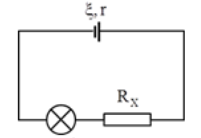
\includegraphics{../figs/VN11-2021-PH-TP014-1}
		\end{center}
	Biết $\calE = \SI{12}{V}$, $r=\SI{4}{\Omega}$, bóng đèn thuộc loại 6 V - 6 W. Để đèn sáng bình thường thì giá trị của $R_x$ là
		\begin{mcq}(4)
			\item $\SI{4}{\Omega}$.
			\item $\SI{2}{\Omega}$.
			\item $\SI{6}{\Omega}$.
			\item $\SI{12}{\Omega}$.
		\end{mcq}
		
	}
	\loigiai
	{	\textbf{Đáp án: B.}
		
		Điện trở của đèn:
		$$R_\text{đ} = \SI{6}{\Omega}.$$
		
		Cường độ dòng điện định mức của đèn:
		$$I_\text{đm} = \SI{1}{A}.$$
		
		Để đèn sáng bình thường thì
		$$I= I_\text{đm} \Rightarrow \dfrac{\calE}{R_x + R_\text{đ} + r} = 1 \Rightarrow R_x = \SI{2}{\Omega}.$$
	}
	\item \mkstar{4}
	
	\cauhoi
	{Cho mạch điện như hình vẽ.
		\begin{center}
			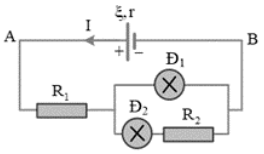
\includegraphics{../figs/VN11-2021-PH-TP014-1-2}
		\end{center}
	Cho biết $\calE = \SI{6.6}{V}$, điện trở trong $r=\SI{0.12}{\Omega}$, bóng đèn Đ1 loại 6 V - 3 W, bóng đèn Đ2 loại $\SI{2.5}{V}$ - $\SI{1.25}{W}$. Coi điện trở của bóng đèn không thay đổi. Các đèn sáng thế nào so với định mức?
		\begin{mcq}(2)
			\item Đ1 sáng yếu, Đ2 sáng mạnh.
			\item Đ1 sáng mạnh, Đ2 sáng yếu.
			\item Cả hai đèn đều sáng yếu.
			\item Cả hai đèn đều sáng mạnh.
		\end{mcq}
		
	}
	\loigiai
	{	\textbf{Đáp án: A.}
		
		Điện trở Đ1:
		$$R_\text{đ1} = \SI{12}{\Omega}.$$
		
		Điện trở Đ2:
		$$R_\text{đ2} = \SI{5}{\Omega}.$$
		
		Cường độ dòng điện định mức qua Đ1:
		$$I_\text{đ1} = \SI{0.5}{A}.$$
		
		Cường độ dòng điện định mức qua Đ2:
		$$I_\text{đ2} = \SI{0.5}{A}.$$
		
		Tính:
		$$R_\text{đ1-đ2-R2} = \SI{4}{\Omega} \Rightarrow R= R_1 + R_\text{đ1-đ2-R2} = \SI{4.48}{\Omega} \Rightarrow I = \dfrac{\calE}{R+r} = \xsi{\dfrac{33}{23}}{A}.$$
		
		Tính cường độ dòng điện qua mỗi đèn:
		$$I_1 = \dfrac{I \cdot R_\text{đ1-đ2-R2}}{R_\text{đ1}} = \xsi{\dfrac{11}{23}}{A}.$$
		
		$$I_2 = \dfrac{I \cdot R_\text{đ1-đ2-R2}}{R_\text{đ2}+R_2} = \xsi{\dfrac{22}{23}}{A}.$$
		
		Vậy đèn 1 sáng yếu hơn định mức và đèn 2 sáng mạnh hơn định mức.
	}
\end{enumerate}

\whiteBGstarEnd

\loigiai
{
	\begin{center}
		\textbf{BẢNG ĐÁP ÁN}
	\end{center}
	\begin{center}
		\begin{tabular}{|m{2.8em}|m{2.8em}|m{2.8em}|m{2.8em}|m{2.8em}|m{2.8em}|m{2.8em}|m{2.8em}|m{2.8em}|m{2.8em}|}
			\hline
			1.D  & 2.A  & 3.C  & 4.D  & 5.D  & 6.D  & 7.C  & 8.C  & 9.C  & 10.A  \\
			\hline
			11.A  & 12.D  & 13.B  & 14.A  & 15.D  & 16.A  & 17.C  & 18.D  & 19.B  & 20.A  \\
			\hline
		\end{tabular}
	\end{center}
}
\section{Tự luận}
\begin{enumerate}[label=\bfseries Câu \arabic*:]
	\item \mkstar{1}
	
	\cauhoi{
		Định luật Ôm đối với toàn mạch đề cập tới loại mạch điện kín nào? Phát biểu định luật và viết biểu thức của định luật.
	}
	
	\loigiai{
		
		Định luật Ôm đối với toàn mạch đề cập tới mạch điện gồm một nguồn điện $(\calE , r)$ mắc với các điện trở ngoài $R$.
		
		Phát biểu định luật: Cường độ dòng điện chạy trong mạch kín tỉ lệ thuận với suất điện động của nguồn điện và tỉ lệ nghịch với điện trở toàn phần của mạch đó.
		
		Biểu thức định luật: $$I=\dfrac{\calE}{R+r}.$$
	}
	
	\item \mkstar{2}
	
	\cauhoi{
		Điện trở trong của một ắcquy là $\SI{0.06}{\Omega}$ và trên vỏ của nó có ghi 12 V. Mắc vào hai cực của ắcquy này một bóng đèn có ghi 12 V - 5 W. Coi điện trở của bóng đèn không thay đổi. Hiệu suất của nguồn điện là bao nhiêu?
	}
	
	\loigiai{
		
		Điện trở trong của bóng đèn:
		$$R=\dfrac{U_\text{đm}^2}{\calP_\text{đm}}=\SI{28.8}{\Omega}.$$
		
		Hiệu suất của nguồn điện:
		$$H=\dfrac{I^2 R}{I^2 (R+r)} = \SI{99.8}{\percent}.$$
	}
	\item \mkstar{3}
	
	\cauhoi{
		Khi mắc điện trở $R_1=\SI{500}{\Omega}$ vào hai cực của một pin mặt trời thì hiệu điện thế mạch ngoài là $U_1=\SI{0.10}{V}$. Nếu thay điện trở $R_1$ bằng điện trở $R_2=\SI{1000}{\Omega}$ thì hiệu điện thế mạch ngoài bây giờ là $U_2=\SI{0.15}{V}$. Tính suất điện động và điện trở trong của pin.
	}
	
	\loigiai{
		
		Áp dụng định luật Ôm:
		$$U_R = IR = \dfrac{\calE}{1 + \dfrac{r}{R}}.$$
		
		Giải phương trình trên, tính được:
		$$\calE = \SI{0.3}{V};$$
		$$r=\SI{1000}{\Omega}.$$
	}
	\item \mkstar{4}
	
	\cauhoi{
		Mạch kín gồm nguồn điện $\calE = \SI{200}{V}$, $r=\SI{0.5}{\Omega}$ và hai điện trở $R_1=\SI{100}{\Omega}$, $R_2=\SI{500}{\Omega}$ mắc nối tiếp. Một Vôn kế không lí tưởng (có điện trở $R_V$) được mắc song song với $R_2$ thì số chỉ của nó là 160 V. Tìm số chỉ của Vôn kế nếu nó được mắc song song với $R_1$.
	}
	
	\loigiai{
		
		\begin{itemize}
		\item Khi Vôn kế mắc song song với $R_2$:
		\begin{center}
			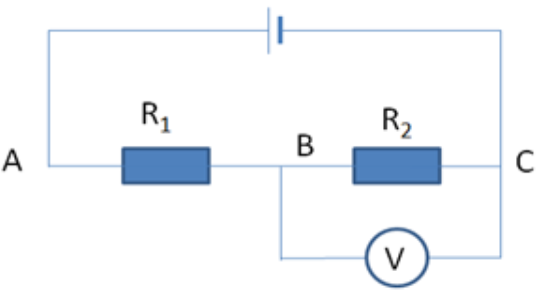
\includegraphics[scale=0.6]{../figs/VN11-2021-PH-TP014-3}
		\end{center}
			
			Mạch gồm $R_1$ nối tiếp ($R_2$ song song $R_V$). Khi đó:
			$$R=R_1 + R_{2V} = \SI{100}{\Omega} + \dfrac{500 R_V}{500 + R_V}.$$
			
			Cường độ dòng điện qua mạch:
			$$I=\dfrac{\calE}{R+r} \Rightarrow U_V = I R_{2V} = \SI{160}{V} \Rightarrow R_V = \SI{2051}{\Omega}.$$
			
		\item Khi Vôn kế mắc song song với $R_1$:
		\begin{center}
			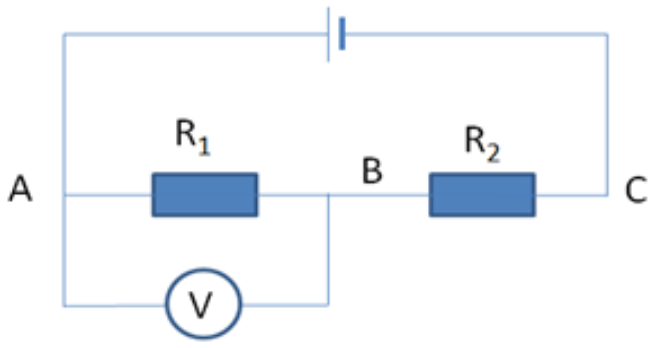
\includegraphics[scale=0.5]{../figs/VN11-2021-PH-TP014-4}
		\end{center}
	
		Mạch gồm $R_2$ nối tiếp ($R_1$ song song $R_V$). Khi đó:
		$$R'=R_2 + R_{1V} = \SI{595.45}{\Omega}.$$
		
		Cường độ dòng điện trong mạch:
		$$I' = \dfrac{\calE}{R' + r} = \SI{0.336}{A}.$$
		
		Số chỉ Vôn kế khi đó:
		$$U_V = I R_{1V} = \SI{32.04}{V}.$$
		\end{itemize}
	}
	\item \mkstar{4}
	
	\cauhoi{
		Cho mạch điện như hình vẽ.
		\begin{center}
			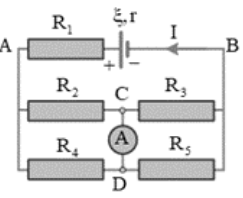
\includegraphics{../figs/VN11-2021-PH-TP014-1-2-3}
		\end{center}
	Cho biết $\calE = \SI{6}{V}$, $r=\SI{0.5}{\Omega}$, $R_1 = R_2 = \SI{2}{\Omega}$, $R_3=R_5 = \SI{4}{\Omega}$, $R_4=\SI{6}{\Omega}$. Điện trở của Ampe kế và dây nối không đáng kể. Tìm số chỉ của Ampe kế.
	}
	
	\loigiai{
		
		Mạch ngoài gồm: $R_1$ nối tiếp ($R_2$ song song $R_4$) nối tiếp ($R_3$ song song $R_5$).
		
		Tính: $R_{24} = \SI{1.5}{\Omega}$, $R_{35} = \SI{2}{\Omega}$. Suy ra $R=R_1 + R_{24} + R_{35} = \SI{5.5}{\Omega}$. Suy ra:
		$$I=\dfrac{\calE}{R+r} = \SI{1}{A}.$$
		
		Tính: $U_{24} = U_2 = I_2 R_2$, suy ra:
		$$I_2 = I \dfrac{R_{24}}{R_2} = \SI{0.75}{A}.$$
		
		Tính $U_{35} = U_3 = I_3 R_3$, suy ra:
		$$I_3 = I \dfrac{R_{35}}{R_3} = \SI{0.5}{A}.$$
		
		Do $I_2 > I_3$ nên $I_A = I_2 - I_3 = \SI{0.25}{A}$.
	}
	
\end{enumerate}